%//==============================--@--==============================//%

\noindent O díodo é um dispositivo eletrónico de dois terminais que pode ser utilizado como elemento básico não-linear para realizar circuitos variados com especial incidência nos conversores de potência que transformam a tensão alternada da rede de distribuição de energia elétrica nas tensões contínuas necessárias para a alimentação de diversos equipamentos de cariz eletrónico.

%//==============================--@--==============================//%
\subsection[2.1 Díodos de junção]{\hspace*{0.075 em}\raisebox{0.2 em}{$\pmb{\drsh}$} Díodos de junção}
\label{subsec:junction-diode}
\noindent O díodo possui dois terminais, ânodo e cátodo, provenientes do contacto metálico entre os dois semicondutores. O sentido ilustrado é o de $p$ para $n$. Designaremos por $i_D$ a corrente e por $v_D$ a tensão que atravessam o díodo.

\begin{figure}[H]
    \centering
    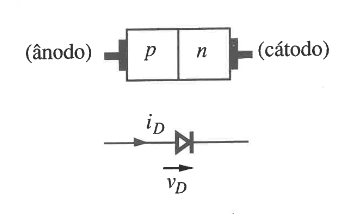
\includegraphics[width = 0.45\linewidth]{img/2/diode.png}
    \caption{Díodo de junção.}
    \label{fig:diode}
\end{figure}

\noindent A característica do díodo, isto é, a relação entre a corrente e a tensão $i_D(v_D)$ pode ser seccionada em 3 zonas de operação, mediante a polarização aplicada\footnotemark:

\vspace{-0.5 em}
\begin{figure}[H]
    \centering
    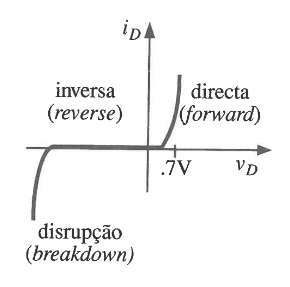
\includegraphics[width = 0.4\linewidth]{img/2/curve.png}
    \caption{Característica do díodo de junção.}
    \label{fig:curve}
\end{figure}

\begin{itemize}
    \item \textbf{Zona de disrupção:} $v_D < 0$ e $v_D$ excede um valor específico de forma a que $i_D < 0$. Possui um comportamento indesejável com exceção nos díodos de Zener, que operam exclusivamente nesta zona.
    \item \textbf{Zona inversa:} $v_D < 0$ e $i_D = 0$. O circuito diz-se cortado.
    \item \textbf{Zona direta:} $v_D > 0$ e $i_D > 0$. O circuito conduz.
    \end{itemize}

%---footnote---%
\footnotetext{Quando $v_D > 0$ diz-se que o díodo possui polarização direta e quando $v_D < 0$ diz-se que possui polarização inversa.}
%---footnote---%

\newpage
\noindent A curva característica possui a seguinte fórmula:
$$
    \boxed{i_D = I_s(e^{v_D/nV_T} - 1)}
$$
\begin{itemize}
    \item[$\pmb{I_s \rightarrow}$] Corrente inversa de saturação. Proporcional à área de junção $pn$.
    \item[$\pmb{V_T \rightarrow}$] Tensão térmica. $V_T = k T/ q$ onde $k$ é a constante de Boltzman, $T$ a temperatura absoluta (tipicamente $T = 300$K) e $q$ a carga do eletrão (\hyperref[subsec:current-flow-semiconductors]{como definido acima}).
    \item[$\pmb{n \rightarrow}$] Coeficiente dependente do material e dimensão do díodo. $1 < n < 2$ onde $n = 2$ quando o díodo é considerado como um componente discreto e $n \simeq 1$ enquanto componente integrado.
\end{itemize}

\noindent\textbf{Nota:} Normalmente $v_D \gg n V_T$ e portanto é considerada a seguinte aproximação:
$$
    \boxed{i_D \simeq I_s e^{v_D/nV_T}}
$$
Mediante esta fórmula podemos tomar as seguintes aproximaçãos:
\begin{itemize}
    \item O díodo permanece cortado para $v_D < 0.5$V.
    \item O díodo conduz para $v_D > 0.7$V.
\end{itemize}

%//==============================--@--==============================//%
\subsubsection[2.1.1 Aproximação linear por troço]{$\pmb{\rightarrow}$ Aproximação linear por troço}

\noindent Assim, é fácil estabelecer uma \textbf{aproximação linear por troço} da característica dos díodos. Com um grau crescente de complexidade (e, consequentemente de rigor) podem considerar-se as três formas de aproximação:

\vspace{0.5 em}
\begin{center}
    \begin{minipage}{0.6\textwidth}
        \begin{itemize}[leftmargin=*]
        \item[] \textbf{\emph{Díodo ideal}}: Num circuito em que o nível de tensões é $\gg v_D = 0.7$V podemos desprezar $v_D$. Desta forma, para $v_D < 0$, $i_D = 0$ e para $i_D > 0$, $v_D = 0$. O díodo é equivalente a um circuito aberto na primeira instância e a um curto circuito na segunda. 
        \end{itemize}
    \end{minipage}%
    \hfill
    \begin{minipage}{0.4\textwidth}
        \begin{center}
            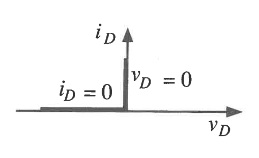
\includegraphics[width=0.9\textwidth]{img/2/ideal.png}
            \label{img:ideal}
        \end{center}
    \end{minipage}
\end{center}

\begin{center}
    \begin{minipage}{0.6\textwidth}
        \begin{itemize}[leftmargin=*]
        \item[] \textbf{\emph{Díodo com tensão constante}}: Admite-se que quando o díodo conduz $v_D = 0.7$V, sendo $i_D = 0$ para $v_D < 0$. O díodo é representado pelo esquema equivalente da \hyperref[fig:tensao-const-esquema]{Fig.\;4 (a)}, constituído por um díodo ideal em série com um gerador de tensão de $V_D = 0.7$V.
        \end{itemize}
    \end{minipage}%
    \hfill
    \begin{minipage}{0.4\textwidth}
        \begin{center}
            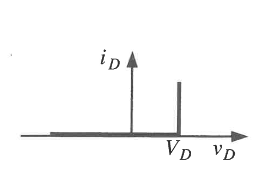
\includegraphics[width=0.9\textwidth]{img/2/tensao-const.png}
            \label{img:tesao-const}
        \end{center}
    \end{minipage}
\end{center}

\begin{center}
    \begin{minipage}{0.6\textwidth}
        \begin{itemize}[leftmargin=*]
        \item[] \textbf{\emph{Díodo com resistência incremental}}: A carac- terística passa a ser aproximada por dois troços de reta. O esquema equivalente (\hyperref[fig:resi-esquema]{Fig.\;4 (b)}) passa a ser constituído por um díodo ideal em série com um gerador de tensão, $V_{D0} \ge 0.5$V, e com resistência incremental, correspondente ao inverso da inclinação da característica: $\Delta v_D/ \Delta i_D$.
        \end{itemize}
    \end{minipage}%
    \hfill
    \begin{minipage}{0.4\textwidth}
        \begin{center}
            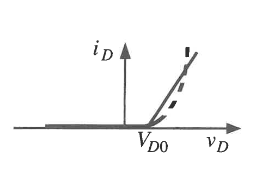
\includegraphics[width=0.9\textwidth]{img/2/resis.png}
            \label{img:resis}
        \end{center}
    \end{minipage}
\end{center}

\begin{figure}[ht] 
    \begin{subfigure}[b]{0.5\linewidth}
        \centering
        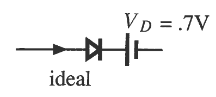
\includegraphics[width=0.5\linewidth]{img/2/tensao-const--esquema.png}
        \caption{Esquema equivalente para o modelo de tensão constante.} 
        \label{fig:tensao-const-esquema} 
        \vspace{1ex}
    \end{subfigure}%% 
    \begin{subfigure}[b]{0.5\linewidth}
        \centering
        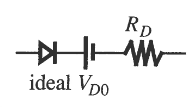
\includegraphics[width=0.5\linewidth]{img/2/resi-esquema.png} 
        \caption{Esquema equivalente para o modelo de resistência.} 
        \label{fig:resi-esquema} 
        \vspace{1ex}
    \end{subfigure} 
    \caption{Esquemas equivalentes das aproximações lineares por troço.}
    \label{fig:esquema}
\end{figure}

%//==============================--@--==============================//%
\subsubsection[2.1.2 Rede resistiva com um só díodo]{$\pmb{\rightarrow}$ Rede resistiva com um só díodo}

\noindent A análise de uma rede resistiva com um só díodo, pode fazer-se com relativa facilidade se se usar o teorema de Thévenin se substituir a rede “vista” pelo díodo pelo seu esquema equivalente de aproximação linear. As variáveis $v_D$, e $i_D$, têm que satisfazer a característica do díodo e têm também que satisfazer a equação que resulta da lei das tensões aplicada ao circuito:

\vspace{-1 em}
\begin{figure}[H]
    \centering
    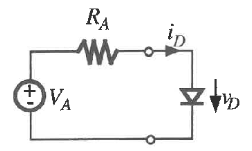
\includegraphics[width = 0.45\linewidth]{img/2/resi-diode-net.png}
    \caption{Rede resistiva com um só díodo.}
    \label{fig:resi-diode-net}
\end{figure}

\vspace{-1 em}
$$
    \boxed{V_A = R_A i_D + v_D}
$$

\paragraph[2.1.2.1 Reta de Carga]{$\pmb{\star}$ Reta de carga}\mbox{}\\[4pt]
\noindent $V_D$ e $I_D$ podem ser determinados fazendo uso de um \textbf{método gráfico}:

\vspace{-1.25 em}
\begin{figure}[H]
    \centering
    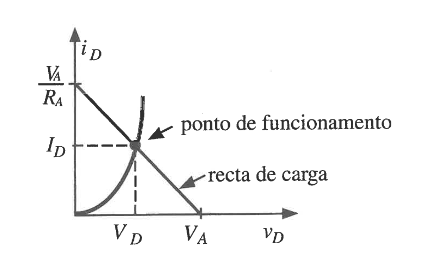
\includegraphics[width = 0.5\linewidth]{img/2/reta-carga.png}
    \caption{Método gráfico: reta de carga.}
    \label{fig:reta-carga}
\end{figure}

\noindent A \textbf{reta de carga} pode ser facilmente traçada através da interseção com os eixos:
$$
    \left.
    \begin{aligned}
        v_D = V_A\quad &\text{e}\quad i_D = 0  \\
        v_D = 0\quad   &\text{e}\quad i_D = V_A/R_A 
    \end{aligned} 
    \;\right\}
    \mkern12mu \begin{minipage}{0.6\textwidth}
                    O \underline{ponto de funcionamento}, oriundo da interseção da reta com a curva característica do díodo, possui as coordenadas de $I_D$ e $V_D$.
              \end{minipage}
$$

\newpage
\paragraph[2.1.2.2 Método iterativo]{$\pmb{\star}$ Método iterativo}\mbox{}\\[4pt]
A análise do circuito pode também ser realizada com recurso a um método iterativo. Invertendo a equação da curva característica simplificada do díodo obtemos:
$$
    v_D \simeq n V_T \ln(i_D/I_s)
$$
Recorrendo a dois possíveis pontos de coordenadas $(v_{DX}, i_{DX})$ e  $(v_{DY}, i_{DY})$ obtemos a seguinte relação:

\vspace{-2em}
\begin{align*}
    v_{DY} &\simeq v_{DX} + n V_T \ln(i_{DY}/i_{DX}) \\
    i_{DY} &= (V_A - V_{DX})/R_A
\end{align*}

\noindent Para aplicar o método iterativo parte-se de uma estimativa $i_{D0}$ e admite-se que a tensão correspondente é $0.7$V. A partir daí aplica-se as duas equações supramencionadas alternadamente:
\begin{empheq}[box=\widefbox]{align*}
        i_{D0} &= \textbf{estimativa}\\
        v_{DY} &= 0.7\text{V}\\
        i_{D1} &= (V_A - V_{D0})/R_A\\
        v_{D1} &\simeq v_{D0} + n V_T \ln{(i_{D1}/i_{D0})}\\
        i_{D2} &= (V_A - V_{D1})/R_A\\
        v_{D2} &\simeq v_{D1} + n V_T \ln{(i_{D2}/i_{D1})}\\
        &\mkern64mu \pmb{\cdots}
\end{empheq}

%//==============================--@--==============================//%
\subsection[2.2 Díodo Zener]{\hspace*{0.075 em}\raisebox{0.2 em}{$\pmb{\drsh}$} Díodo Zener}
\label{subsec:zener-diode}

A íngreme curva $i-v$ destes díodos na \textit{breakdown region} (\hyperref[fig:zener-diode]{Fig. 9 (a)}), indica uma queda de tensão quase constante\footnotemark[2]---algo que sugere o seu uso em reguladores de tensão.

\vspace{-0.5em}
\begin{figure}[H]
    \begin{subfigure}{0.5\textwidth}
        \centering
        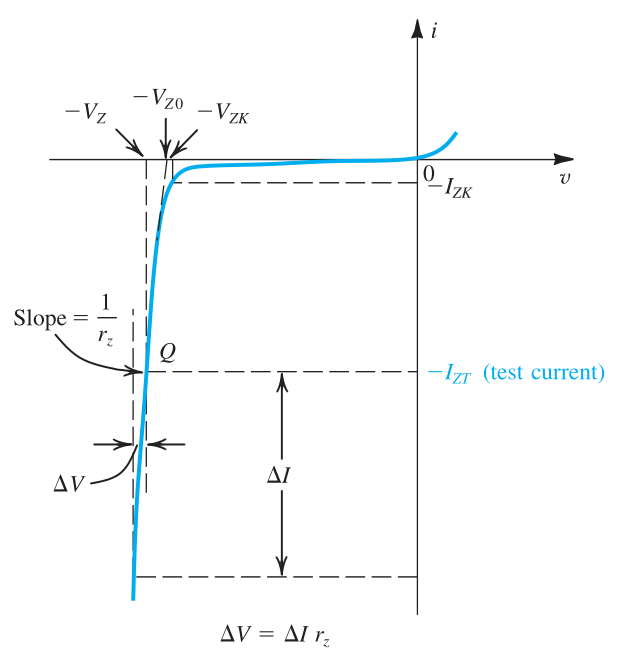
\includegraphics[width=\linewidth]{img/2/zener-diode-iv.png}
        \caption{``The diode i–v characteristic (...)''\cite{sedra-smith:microelectronic-circuits}}
    \end{subfigure}
    \begin{subfigure}{0.45\textwidth}
        \centering
        \raisebox{10.78em}{
            \begin{minipage}{\textwidth}
                \begin{minipage}{\textwidth}
                    \centering
                    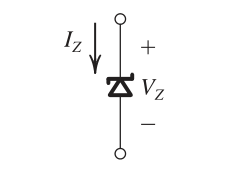
\includegraphics[width=0.6\linewidth]{img/2/zener-diode.png}
                    \caption{``Circuit symbol for a zener diode.''\cite{sedra-smith:microelectronic-circuits}}
                \end{minipage}
                \begin{minipage}{\textwidth}
                    \centering
                    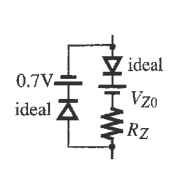
\includegraphics[width=0.45\linewidth]{img/2/zener-diode-model.png}
                    $$
                        \boxed{ V_Z = V_{Z0} + r_Z I_Z }
                    $$
                    \caption{``Esquema equivalente com resistência.''\cite{medeiros:ICEE}}
                \end{minipage}
            \end{minipage}
        }
    \end{subfigure}
    \caption{Díodo Zener: conhecidos como díodos de rutura ou zener; normalmente têm o cátodo positivo (com a corrente a fluir para este), o que resulta em \underline{valores positivos para $I_Z$ e $V_Z$} na prática, como indica o esquema equivalente (c).}
    \label{fig:zener-diode}
\end{figure}

\footnotetext[2]{%
    Para correntes superiores à corrente de joelho (\textit{knee current}) $I_{ZK}$, a característica $i-v$ do diodo zener é quase linear. O fabricante normalmente especifica a tensão $V_Z$ num dado $I_{ZT}$ (a corrente de teste).
}
%//==============================--@--==============================//%